%
% crit.tex
%
% (c) 2018 Prof Dr Andreas Müller, Hochschule Rapperswil
%
\section{Gleichgewichtslösungen und kritische Punkte}
\rhead{Gleichgewichtslösungen}
Wir gehen in diesem Abschnitt von einer autonomen Differentialgleichung
der Form
\begin{equation}
\frac{dx}{dt} = f(x)
\label{skript:dgl:gleichung}
\end{equation}
aus
mit einer Funktion $f\colon \mathbb R^n \to \mathbb R^n$.
Die Funktion $f$ wird im Allgemeinen von weiteren Parametern abhängen
wie zum Beispiel dem $\text{CO}_2$-Gehalt der Atmosphäre oder der Salinität
der Meere.
Sofern nötig machen wir diese mit der Schreibweise $f(x,p)$ mit
$p\in\mathbb R^m$ explizit sichtbar.

\begin{definition}
Ein Punkt $x_0\in\mathbb R^n$ heisst {\em Gleichgewichtslösung}
wenn die konstante Funktion $x(t)=x_0$ eine Lösung der
Differentialgleichung~\ref{skript:dgl:gleichung} ist.
\index{Gleichgewichtslösung}
\end{definition}

Eine Gleichgewichtslösung hat $\dot{x}(t)=0$ und ist daher eine
Nullstelle der Funktion $f$,
$f(x_0)=0$.
\begin{definition}
Eine Nullstelle von $f$ heisst {\em kritischer Punkt} der
Differentialgleichung~\ref{skript:dgl:gleichung}.
\end{definition}
\index{kritischer Punkt}%

Wenn $f$ ausserdem von den Parametern $p\in\mathbb R^m$ abhängt,
wird auch die Menge der Nullstellen von $f$ von $p$ abhängen.
Wir schreiben
\[
N(p) = \{x\in\mathbb R^n\;|\; f(x,p)\}
\]
für die Menge der Nullstellen. 
Im Allgemeinen werden sich die Mengen $N(p)$ für verschiedene $p$ 
unterscheiden.

Sei also $p_0\in\mathbb R^m$ ein Parametervektor und $x_0$ eine
Gleichgewichtslösung von $f$, also $f(x_0,p_0)=0$.
Unter zusätzlichen Annahmen über die Funktion $f$ kann man zeigen,
dass $x_0$ in einer Umgebung von $p_0$ zu einer Funktion
$x_0(p)$ erweitert werden kann, derart dass $x_0(p)$ jeweils ein
kritischer Punkt von $f$ ist für die Parameterwerte $p$, also
$f(x_0(p),p)=0$.
Diese Theorie ist für allerdings nicht besonders nützlich, denn
sie sagt uns nur, dass sich kritische Punkte stetig in Abhängigkeit vom
Parametervektor bewegen.
Besonders interessant für die Diskussion des Klimawandels sind
Fälle, wo Gleichgewichtslösungen sich sprunghaft ändern, wie wir in
Abschnitt~\ref{subsection:budyko} diskutieren werden.

\subsection{Stabilität}
Wir betrachten eine Gleichgewichtslösung $x(t)=x_0$ der Differentialgleichung
\eqref{skript:dgl:gleichung}.
\begin{definition}
Die Gleichgewichtslösung $x(t)=x_0$ heisst stabil, wenn eine Lösung zu
einer Anfangsbedingung $\bar x_0$, die $|x_0-\bar x_0|<\varepsilon$
erfüllt, für alle Zeiten nahe bei $x_0$ bleibt, also
$|\bar x(t)- x_0|<\varepsilon$.
\end{definition}
\index{Stabilität}%

\begin{beispiel}
Wir betrachten die Differentialgleichung
\[
\frac{dx}{dt} = ax.
\]
Sie hat die Gleichgewichtslösung $x(t)=0$.
Eine Lösung, die die Anfangsbedingung $x(0)=\varepsilon$ erfüllt, 
ist $x(t)=\varepsilon e^{at}$, denn
\[
\frac{d}{dt}
\varepsilon e^{at}
=
a\varepsilon e^{at}.
\]
Wenn $a>0$, dann wächst die Lösung exponentiell an, die Gleichgewichtslösung 
ist als nicht stabil.
Für $a<0$ dagegen nimmt $x(t)=\varepsilon e^{at}$ exponentiell schnell ab,
die Gleichgewichtslösung ist stabil.
\end{beispiel}

Für eindimensionale Systeme ist Stabilität besonders einfach zu
diskutieren, wir tun dies im Rahmen der Diskussion der wichtigsten
Bifurkationstypen in Abschnitt~\ref{section:bifurkation-eindim}.

\subsection{Zeitumkehr}
\index{Zeitumkehr}%
Wir gehen wieder von der autonomen
Differentialgleichung~\eqref{skript:dgl:gleichung}
mit der Lösung $x(t)$ mit Anfangsbedingung $x_0$ aus.
Ersetzen wir $t$ durch $-s$, erhalten wir die autonome Differentialgleichung
\begin{equation}
-\frac{dx}{ds}
=
f(x),
\end{equation}
mit der gleichen Anfangsbedingung.
Die Funktion $s\mapsto x(-s)$ ist eine Lösung.

Die Zeitumkehr verändert den Stabilitätscharakter einer Gleichgewichtslösung.
Ist $x_0$ eine stabile Gleichgewichtslösung, dann nehmen Lösungen mit
Anfangsbedingungen in der Nähe von $x_0$ nicht weiter zu, sondern
höchstens ab.
Es ist also möglich, dass die Lösung nach Zeitumkehr instabil wird.

Bei zweidimensionalen Systemen ist es aber durchaus möglich, eine
Gleichgewichtslösung in beiden Zeitrichtungen instabil sind.
Als Beispiel betrachten wir das zweidimensionale Differentialgleichungssystem
\begin{equation}
\frac{d}{dt}
\begin{pmatrix}x\\y\end{pmatrix}
=
\begin{pmatrix}1&0\\0&-1\end{pmatrix}
\begin{pmatrix}x\\y\end{pmatrix}.
\end{equation}
Sie hat die beiden Lösungen
\begin{align*}
x_1(t)&=
\varepsilon \begin{pmatrix}e^t\\0\end{pmatrix}
&&\text{und}&
x_2(t)
&=
\varepsilon \begin{pmatrix}0\\e^{-t}\end{pmatrix}
\end{align*}
zu den Anfangsbedingungen
\begin{align*}
x_1(0)&=\begin{pmatrix}\varepsilon\\0\end{pmatrix}
&&\text{und}&
x_2(0)&=\begin{pmatrix}0\\\varepsilon\end{pmatrix}.
\end{align*}
Die Lösung $x_1(t)$ wächst für $t>0$ exponentiell an, die Gleichgewichtslösung
$x(t)=0$ kann also für $t>0$ nicht stabil sein.
Für $t\to-\infty$ nimmt $x_1(t)$ exponentiell ab, aber trotzdem ist
die Nulllösung nicht stabil, dann die Lösung $x_2(t)$ nimmt für 
$t\to-\infty$ exponentiell zu.

\section{Bifurkationen eindimensionaler Systeme
\label{section:bifurkation-eindim}}
\rhead{Bifurkationen}
In diesem Abschnitt betrachten wir eindimensionale Differentialgleichung
\begin{equation}
\frac{dx}{dt} = f(x,\lambda),
\end{equation}
die ausserdem von einem Parameter $\lambda$ abhängt.
Wir fragen nach den Gleichgewichtslösungen in Abhängigkeit vom
Parameter $\lambda$.

Die nachfolgenden prototypischen Bifurkationen können in vielen
\index{Bifurkation}%
weiteren Differentialgleichungen beobachtet werden. 
Für alle Werte des Parameters ist $0$ ein kritischer Wert,
es gilt also $f(0,\lambda)=0$.
Wir können die $f$ in eine Taylor-Reihe 
\begin{equation}
f(x,\lambda)
=
\sum_{k,l} \frac{1}{(k+l)!}\frac{\partial^{k+l} f(0,0)}{\partial t^k\partial\lambda^l} x^k\lambda^l
=
a_{10}x + a_{01}\lambda
+
a_{20}x^2 + a_{11}x\lambda + a_{02}\lambda^2 + \dots
\end{equation}
entwickeln.
Die verschiedenen Bifurkationen lassen sich charakterisieren durch
die führenden Terme in dieser Entwicklung.
Insbesondere können wir verlangen, dass der führende Term für $\lambda$
immer linear in $\lambda$ sein soll.
Ist dies nämlich nicht der Fall, ist also der führende Term in 
$\lambda$ von der Form $\lambda^\alpha$, ersetzen wir den
Parameter einfach durch $\tau=\lambda^\alpha$.

In den folgenden Beispielen und Abschnitten wird der Parameter $\lambda$
entlang der horizontalen Achse aufgezeichnet, die Position $x$
entlang der vertikalen Achse.
Positive Werte von $f(x,\lambda)$ führen dazu, dass sich mit zunehmender
Zeit die Lösung $x(t)$ nach oben bewegt, solche Punkte werden in den
Diagrammen rot eingefärbt, ausserdem wird mit Pfeilen die Bewegungsrichtung
der Punkte angedeutet.

\begin{beispiel}
\begin{figure}
\centering
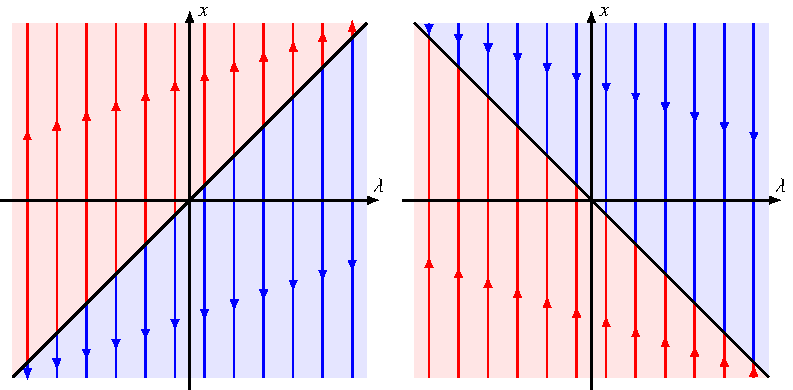
\includegraphics{chapters/3/lin1.pdf}
\caption{
Phasendiagramm der Differentialgleichung $\dot x = x-\lambda$ links und
$\dot x = -x-\lambda$ rechts.
Die Gleichgewichtslösung $x=\lambda$ ist im linken Fall instabil,
während $x=-\lambda$ im rechten Fall eine stabile Gleichgewichtslösung ist.
\label{skript:dgl:phasen1}
}
\end{figure}%
Der einfachste Fall ist bis auf eine Skalierung
\begin{equation}
f(x,\lambda)=x-\lambda.
\label{skript:dgl:linear1}
\end{equation}
$f$ hat nur einen einzigen kritischen Punkt, nämlich $x_0=-\lambda$.
Das Phasendiagramm dafür ist in Abbildung~\ref{skript:dgl:phasen1}
Man erkennt, dass Läsungen, die bei $x$-Werten $x>\lambda$ beginnen,
anwachsen und sich von der Gleichgewichtslösung entfernen.
Umgekehrt nehmen Lösungen ab, die bei $x$-Werten $x<\lambda$ beginnen,
und entfernen sich damit ebenfalls von der Gleichgewichtslösung.
Die Differentialgleichung mit rechter Seite~\ref{skript:dgl:linear1}
hat kein stabile Lösungen.

Die analoge Analyse für die Differentialgleichung
\[
\frac{dx}{dt} = -x-\lambda
\]
ist in Abbildung~\ref{skript:dgl:linear1} dargestellt.
Die Gleichgewichtslösung $x_0=-\lambda$ ist stabil.
\end{beispiel}

Dieses Beispiel zeigt, dass interessante Bifurkationsereignisse
erst dann auftreten, wenn der führende Term in $x$ der Taylor-Entwicklung
von $f$ von höherer als linearer Ordnung ist.


\subsection{Sattel-Knoten-Bifurkation}
\index{Sattel-Knoten-Bifurkation}%
\begin{figure}
\centering
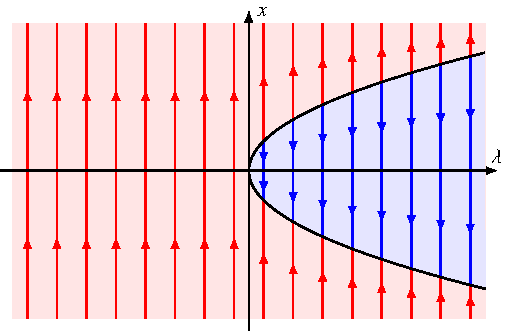
\includegraphics{chapters/3/saddle-node.pdf}
\caption{Phasendiagramm der Sattel-Knoten-Bifurkation zur
Differentialgleichung~\ref{skript:dgl:sattel-knoten-dgl}.
Für $\lambda>0$ gibt es zwei Gleichgewichtslösungen $\pm\sqrt{\lambda}$,
eine ist stabil, die andere instabil.
\label{skript:dgl:saddle-node}}
\end{figure}%
Die {\em Sattel-Knoten-Bifurkation}
\index{Sattel-Knoten-Bifurkation}%
tritt auf in der Differentialgleichung
\begin{equation}
\frac{dx}{dt}=x^2 - \lambda.
\label{skript:dgl:sattel-knoten-dgl}
\end{equation}
Für $\lambda >0$ hat die Gleichung~\ref{skript:dgl:sattel-knoten-dgl}
zwei Gleichgewichtslösungen $\pm\sqrt{\lambda}$.
In Abbildung~\ref{skript:dgl:saddle-node} ist das Phasendiagramm
dargestellt.
Daraus geht hervor, dass die Gleichgewichtslösung $q\sqrt{\lambda}$
instabil ist, während $-\sqrt{\lambda}$ stabil ist.

\subsection{Heugabel-Bifurkation}
\index{Heugabel-Bifurkation}%
\begin{figure}
\centering
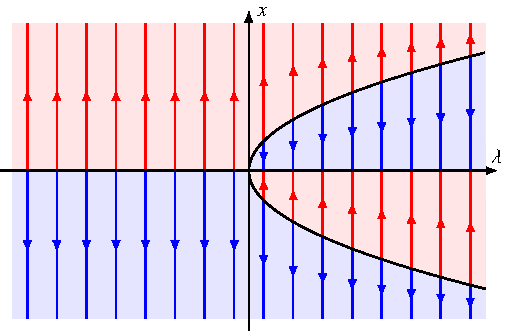
\includegraphics{chapters/3/pitchfork.pdf}
\caption{Phasendiagramm der Heugabel-Bifurkation.
\label{skript:dgl:pitchfork}}
\end{figure}
Die {\em Heugabel-Bifurkation} tritt bei der Differentialgleichung
\begin{equation}
\frac{dx}{dt} = x^3 - \lambda x
\label{skript:dgl:heugabel-dgl}
\end{equation}
auf, bei der der führende Term
dritter Ordnung in $x$ ist.
Die Differentialgleichung
kann auch in der Form
\[
\frac{dx}{dt}
=
x(x^2-\lambda)
\]
geschrieben werden.
Sie hat $0$ als Gleichgewichtslösung für alle $\lambda$.
Für $\lambda>0$ hat sie zusätzlich die Gleichgewichtslösungen
$\pm\sqrt{\lambda}$.

Das Phasendiagramm~\ref{skript:dgl:heugabel-dgl} zeigt, dass
die einzige Gleichgewichtslösung bei $x_0=0$ instabil ist.
Beim Übergang zu $\lambda>0$ wird die Gleichgewichtslösung $x_0=0$
stabil.
Die beiden neuen Gleichgewichtslösungen $\pm\sqrt{\lambda}$ sind
beide instalbil.

Die Differentialgleichung
\[
\frac{dx}{dt} = -x^3+\lambda x
\]
hat die gleichen Gleichgewichtslösungen, jedoch ist $0$ für
$\lambda<0$ eine stabile Lösung, die beim Übergang zu $\lambda>0$
instabil wird.
Die Gleichgewichtslösungen $\pm\sqrt{\lambda}$ für $\lambda >0$
sind stabil.

\subsection{Transkritische Bifurkation}
\index{transkritische Bifurkation}%
\begin{figure}
\centering
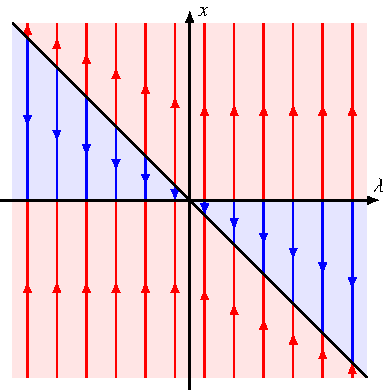
\includegraphics{chapters/3/trans.pdf}
\caption{Phasendiagramm der transkritischen Bifurkation in der
Differentialgleichung~\eqref{skript:dgl:transkritisch-dgl}.
\label{skript:dgl:transfig}}
\end{figure}
Die Differentialgleichung
\begin{equation}
\frac{dx}{dt}
=
x^2 + \lambda x
=
x(x+\lambda)
\label{skript:dgl:transkritisch-dgl}
\end{equation}
hat Gleichgewichtslösung $0$ und $-\lambda$.
Das Phasendiagramm in Abbildung~\ref{skript:dgl:transfig} zeigt, dass 
für $\lambda<0$ die Gleichgewichtslösung $0$ stabil ist, die
Gleichgewichtslösung $-\lambda$ hingegen instabil.
Beim Übergang zu $\lambda>0$ wird die Gleichgewichtslösung $0$ instabil
und die Gleichgewichtslösung $-\lambda$ wird instabil.

\subsection{Ein Beispiel zur globalen Mitteltemperatur\label{subsection:budyko}}
\index{globale Mitteltemperatur}%
\begin{figure}
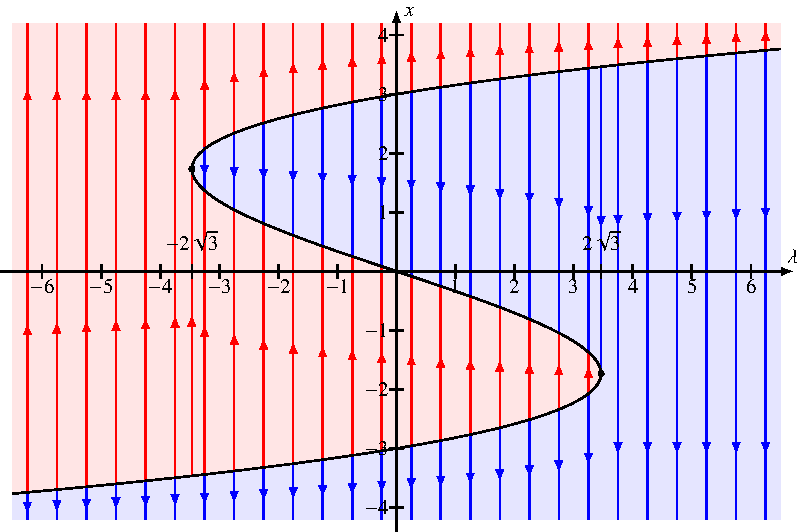
\includegraphics{chapters/3/kubisch.pdf}
\caption{Phasendiagramm der Differentialgleichung~\eqref{skript:dgl:kubisch}.
\label{skript:dgl:kubischfig}}
\end{figure}
Das in Abschnitt~\ref{subsection:modell von budyko} beschriebene
Budyko-Modell versucht, die globale Mittelemperatur in Abhängigkeit
von der Einstrahlung und der Albedo zu modellieren.
Mehr zu diesen Ansätzen wird in Kapitel~5 dargestellt.
\index{Budyko-Modell}

Als Beispiel für die Diskussion eines solchen Modells betrachten wir
die Differentialgleichung
\begin{equation}
\frac{dx}{dt}
=
\frac13(x^3 - 9x) - \lambda.
\label{skript:dgl:kubisch}
\end{equation}
Die Gleichgewichtslösungen sind die Nullstellen der kubischen Gleichung
\[
f(x,\lambda)
=
x^3-9x-3\lambda=0.
\]
Diese sind für beliebiges $\lambda$ nicht so leicht zu finden.
Für $\lambda=0$ sind die kritischen Punkte $0$ und $\pm 3$.
DIe Funktion $f(x)$ hat lokale Minima bei den $\pm\sqrt{3}$ mit
Funktionswerten $\pm2\sqrt{3}$.
Daher gibt es im Interval $(-2\sqrt{3},2\sqrt{3})$ drei 
Gleichgewichtslösungen, ausserhalb jedoch jeweils nur eine.

Das zugehörige Phasendiagramm ist in Abbildung~\ref{skript:dgl:kubischfig}
dargestellt.
Die Gleichgewichtslösungen oben und unten auf der S-Kurve sind instabil,
nur der Ast zwischen den beiden lokalen Extrema von $f(x)$ besteht
aus stabilen Gleichgewichtslösungen.

Wächst der Parameter $\lambda$ über den kritischen Wert $2\sqrt{3}$
hinaus, gibt es keinen stabilen Gleichgewichtszustand mehr, das System
divergiert nach $-\infty$. 
Analog strebt das System gegen $+\infty$ wenn der Parameter den Wert
$-2\sqrt{3}$ unterschreitet.

Die Differentialgleichung 
\begin{equation}
\frac{dx}{dt}
=
-f(x,\lambda)
\label{skript:dgl:kubisch2}
\end{equation}
hat die gleichen Gleichgewichtslösungen wie \eqref{skript:dgl:kubisch},
jedoch sind die stabilen Gleichgewichtslösungen von \eqref{skript:dgl:kubisch}
instabile Gleichgewichtslösungen von \eqref{skript:dgl:kubisch2}
und umgekehrt.
Beim Anstieg des Parameters $\lambda$ über den Wert $2\sqrt{3}$
springt das System, falls es sich im unteren Gleichtszustand befand,
in den oberen.
Sinkt der Wert von $\lambda$ wieder unter $2\sqrt{3}$ wird, bleibt
es jedoch auf dem oberen Gleichgewichtspunkt.


